%!TEX root=../document.tex

\section{Lösungsideen}
Beim Lösen der Aufgaben bin ich auf folgende Methoden gekommen:

\begin{itemize}
	\item Bereits erledigte Aufgaben (A01-A07) kopiert und umgeschrieben mittels der MySQL-Doku
	\item Alle Aufgaben neu schreiben mittels der MySQL-Doku
\end{itemize}

	Im Endeffekt haben mir beide Methoden zum Erfüllen dieser Aufgabe geholfen, wobei ich öfters auf die zweite Art
	zurückgegfriffen habe.
	
	Beispielsweise war es bei A03 nicht anders möglich als die Tabellen mittels einem \textbf{INNER JOIN} zusammen zu führen um so den richtigen Tagesumsatz eines Kellners herauszufinden.
\section{Probleme}
	Während der Importierung von den PostgreSQL-Aufgaben sind keine gröberen Probleme aufgetreten. Lediglich hatte ich ein Problem in meinem CREATE-Script, welches ich schnell lösen konnte. (DROP - Befehl)
\section{Konkrete Umsetzung}
	\subsection{A01}
		Alle Preise sollen so geändert (erhöht) werden, dass sie mit 99 Cent enden!
		\begin{lstlisting}[
		language=SQL,
		showspaces=false,
		basicstyle=\ttfamily,
		numbers=left,
		numberstyle=\tiny,
		commentstyle=\color{gray}
		]
		delimiter //
		CREATE PROCEDURE preis99() 
		BEGIN
		UPDATE speise SET preis=ceil(preis)-0.01;
		END //
		delimiter ;
		
		SELECT * FROM speise;
		CALL preis99();
		SELECT * FROM speise;
		\end{lstlisting}
		
		\clearpage
		
		Alle Rechnung zu denen es keine Bestellung gibt, sollen gelöscht werden.
		
		\begin{lstlisting}[
		language=SQL,
		showspaces=false,
		basicstyle=\ttfamily,
		numbers=left,
		numberstyle=\tiny,
		commentstyle=\color{gray}
		]
		delimiter //
		CREATE PROCEDURE loescheRechnung()
		BEGIN
		delete from rechnung where rnr not in (select rnr from bestellung);
		END // 
		delimiter ;
				
		INSERT INTO rechnung VALUES (10, CURDATE(), 1, 'gedruckt', 1);
				
		SELECT * FROM rechnung;
		CALL loescheRechnung();
		SELECT * FROM rechnung;
				
		\end{lstlisting}
				
	\subsection{A02}
		Erstelle eine Funktion mit zwei Parametern: Alle Speisen die billiger als der Durchschnittspreis 
		aller Speisen sind, sollen um einen fixen Betrag erhöht werden, alle Speisen die teurer sind, sollen um einen Prozentwert erhöht werden.
		
		\begin{lstlisting}[
		language=SQL,
		showspaces=false,
		basicstyle=\ttfamily,
		numbers=left,
		numberstyle=\tiny,
		commentstyle=\color{gray}
		]
		delimiter //
		CREATE PROCEDURE preiserhoehung(IN prozent DECIMAL(30,2),IN abpreis DECIMAL(30,2))
		BEGIN
		DECLARE av DECIMAL DEFAULT (SELECT avg(preis) FROM speise);
		UPDATE speise SET preis = preis * (100 + prozent) / 100 where preis > av;
		UPDATE speise SET preis = preis + abpreis where preis <= av;
		END//
		delimiter ;
			
		SELECT * FROM speise;
		CALL preiserhoehung(10,1.75);
		SELECT * FROM speise;
				
				
		\end{lstlisting}
				\clearpage
	\subsection{A03}
		Der Tagesumsatz für einen bestimmten Kellner soll für den aktuellen Tag ermittelt werden.
		
		\begin{lstlisting}[
		language=SQL,
		showspaces=false,
		basicstyle=\ttfamily,
		numbers=left,
		numberstyle=\tiny,
		commentstyle=\color{gray}
		]
		CREATE FUNCTION tagesumsatz(kel INT) 
		RETURNS DECIMAL(30,2) DETERMINISTIC
		RETURN 
		(select sum(preis*anzahl) from speise 
		inner join bestellung on speise.snr = bestellung.snr 
		inner join rechnung on rechnung.rnr = bestellung.rnr
		where knr=kel AND rechnung.status like 'bezahlt%' AND rechnung.datum = CURDATE());
		
		SELECT tagesumsatz(1);
		SELECT tagesumsatz(2);
		select tagesumsatz(3);
		
		\end{lstlisting}
		

	\subsection{A04}
		Erstelle eine weitere Funktion zur Berechnung der MWSt. Zeige von allen Speisen den Brutto-Preis 
		als Brutto und die darin enthaltene MWSt. als Spalte MWSt an. Zusatz: Die Anzeige bei Brutto/MWSt 
		soll auf zwei Nachkommastellen beschränkt werden.
		\begin{lstlisting}[
		language=SQL,
		showspaces=false,
		basicstyle=\ttfamily,
		numbers=left,
		numberstyle=\tiny,
		commentstyle=\color{gray}
		]
		CREATE FUNCTION bruttoPreis(preis DECIMAL(30,2))
		RETURNS DECIMAL(30,2) DETERMINISTIC
		RETURN
		(SELECT round(preis*1.2, 2));
		delimiter //
		
		CREATE FUNCTION mwstPreis(preis DECIMAL(30,2))
		RETURNS DECIMAL(30,2) DETERMINISTIC
		RETURN
		(SELECT round(preis*0.2, 2));
		delimiter //
		CREATE PROCEDURE ausgabe1()
		BEGIN
		Select bezeichnung, bruttoPreis(speise.preis) as "Brutto", mwst(
		speise.preis*1.2) as "MWST" from speise;
		END //
		delimiter ;
		
		call ausgabe1();
			
		\end{lstlisting}
		
		\clearpage
		
	\subsection{A05}
		Erstelle eine Funktion zur Anzeige der Bezeichnungen der noch nie bestellten Speisen.
		\begin{lstlisting}[
		language=SQL,
		showspaces=false,
		basicstyle=\ttfamily,
		numbers=left,
		numberstyle=\tiny,
		commentstyle=\color{gray}
		]
		delimiter //
		CREATE PROCEDURE nichtbestellt()
		BEGIN
		Select bezeichnung from speise where snr not in (Select snr from bestellung);
		END //
		delimiter ;
		
		call nichtbestellt();
		
		\end{lstlisting}
		
		
		Zusatz: Erweitere die aufrufende SELECT-Anweisung so, dass das Ergebnis als Tabelle mit den Spaltenüberschriften ''Bezeichnung'' und ''Nettopreis'' angezeigt wird.
		als Select nicht möglich, da call procedure nicht in einer select Anweißung aufgerufen werden kann.
		mögliche Variante- neue Procedure 
		
		\begin{lstlisting}[
		language=SQL,
		showspaces=false,
		basicstyle=\ttfamily,
		numbers=left,
		numberstyle=\tiny,
		commentstyle=\color{gray}
		]
		delimiter //
		CREATE PROCEDURE ausgabe2()
		BEGIN
		Select bezeichnung, preis as "Nettopreis" from speise where bezeichnung in (Select bezeichnung from speise where snr not in (Select snr from bestellung));
		END //
		delimiter ;
				
		call ausgabe2();
				
		\end{lstlisting}
		
		\clearpage
	\subsection{A06}
		Erstelle zwei Funktionen die in der SELECT-Klausel eingebettet werden, um damit zusätzliche Spalten je Kellner anzeigen zu können. Die aufrufende SELECT-Anweisung soll folgende Ausgabe produzieren:
		Kellnername, Anzahl der Rechnungen, Status der spätesten Rechnung
		
		\begin{lstlisting}[
		language=SQL,
		showspaces=false,
		basicstyle=\ttfamily,
		numbers=left,
		numberstyle=\tiny,
		commentstyle=\color{gray}
		]
		CREATE FUNCTION anzahlrechnungen(kel INTEGER)
		RETURNS BIGINT DETERMINISTIC
		RETURN
		(SELECT count(rechnung.knr) 
		FROM rechnung
		WHERE rechnung.knr = kel);
		
		CREATE FUNCTION letzteRechnung(kel INTEGER)
		RETURNS CHAR(8) DETERMINISTIC
		RETURN
		(select status from rechnung where datum = (select max(datum) from rechnung where rechnung.knr = kel) and rechnung.knr = kel limit 1);
		
		delimiter //
		CREATE PROCEDURE ausgabe3()
		BEGIN
		Select distinct kellner.name, anzahlrechnungen(rechnung.knr) as 'Anzahl Rechnungen', letzterechnung(rechnung.knr) as 'Letzte Rechnung' from rechnung inner join kellner on kellner.knr = rechnung.knr order by kellner.name asc;
		END //
		delimiter ;
		
		call ausgabe3();
		
			
		\end{lstlisting}
		\clearpage
	\subsection{A07}
		Es soll eine Liste der Kellner und deren jeweiliger Tagesumsatz ausgegeben werden.
		Korrekte Lösung mit der Original-DB: nur eine Zeile mit Kellner1 und 71.00
		
		\begin{lstlisting}[
		language=SQL,
		showspaces=false,
		basicstyle=\ttfamily,
		numbers=left,
		numberstyle=\tiny,
		commentstyle=\color{gray}
		]
		delimiter //
		CREATE PROCEDURE umsatzkellner()
		BEGIN
		select kellner.name,  sum(preis*anzahl) from kellner
		inner join rechnung on kellner.knr = rechnung.knr 
		inner join bestellung on rechnung.rnr = bestellung.rnr
		inner join speise on speise.snr = bestellung.snr 
		where rechnung.status = 'bezahlt' AND rechnung.datum = current_date
		group by kellner.knr;
		END //
		delimiter ;
		
		call umsatzkellner();
			
			
		\end{lstlisting}
		
		
		
\section{Beweis der Umsetzung}
	Umsetzung folgender Aufgabe: \textbf{A02}
	\begin{figure}[!h]
		\begin{center}
			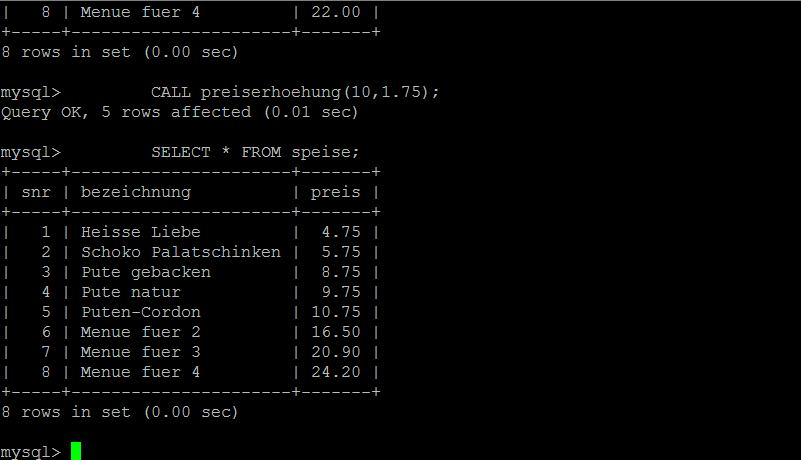
\includegraphics[width=0.7\textwidth]{images/A02}
			\caption{Screenshot der Konsole beim Durchführen von A02}
			\label{broker}
		\end{center}
	\end{figure}
	\clearpage
	Umsetzung folgender Aufgabe: \textbf{A06}
	\begin{figure}[!h]
		\begin{center}
			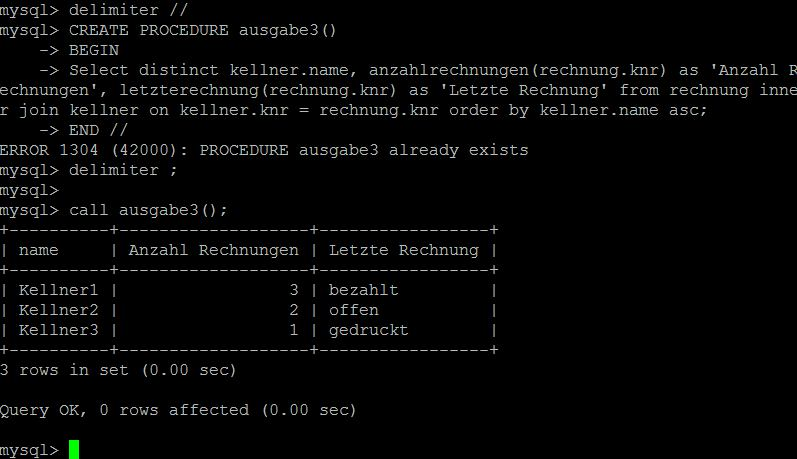
\includegraphics[width=0.7\textwidth]{images/A06}
			\caption{Screenshot der Konsole beim Durchführen von A06}
			\label{broker}
		\end{center}
	\end{figure}
	\newline
	Umsetzung folgender Aufgabe: \textbf{A05}
	\begin{figure}[!h]
		\begin{center}
			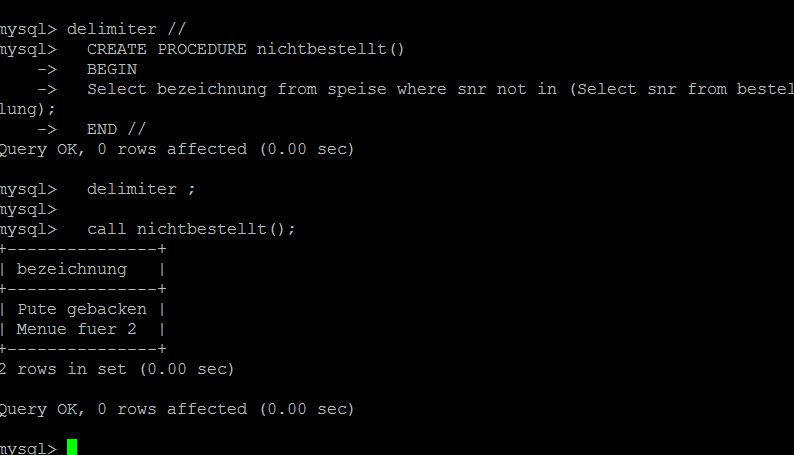
\includegraphics[width=0.7\textwidth]{images/A05}
			\caption{Screenshot der Konsole beim Durchführen von A05}
			\label{broker}
		\end{center}
	\end{figure}
	
	